\section{\label{sec:Introduction} Introduction}
	
Aging is an important non-Markovian effect in binary-state models that has significant implications. It describes how the persistence time of an agent in a particular state influences the transition rate to a different state \cite{stark-2008, fernandez-gracia-2011, perez-2016, boguna-2014, chen-2020}. As such, the longer an agent remains in the current state, the smaller the probability of changing. Aging has been shown to cause coarsening dynamics towards a consensus state in the Voter model \cite{fernandez-gracia-2011,peralta-2020C}, to induce bona fide continuous phase transitions in the noisy Voter model \cite{artime-2018,peralta-2020A}, modify the phase diagram and non-equilibrium dynamics of the Schelling segregation model \cite{Abella-2022}, and to modify non-trivially the cascade dynamics of the threshold model \cite{Abella-2022-AME}. The introduction of aging is motivated by strong empirical evidence that human interactions do not occur at a constant rate and cannot be described using a Markovian assumption. Empirical studies have reported heavy-tail inter-event time distributions that reflect heterogeneous temporal activity patterns in social interactions \cite{karsai-2011, rybski-2009, zignani-2016, artime-2017, kumar-2020}.
	
In this work, we present a comprehensive analysis of the Symmetrical Threshold model, including its full phase diagram, and we investigate the effects of aging in the model. The model is examined in various network topologies, such as the complete graph, Erd\H{o}s-Rényi (ER)  \cite{erdos1960evolution}, random regular (RR) \cite{wormald1999models}, and a two-dimensional Moore lattice. The possible phases of the system are defined by the final stationary state as well as by the ordering/disordering dynamics characterized by the time-dependent magnetization, interface density, persistence, and mean internal time. For both the original model and the aging variant, the results of Monte Carlo numerical simulations are compared with results from the theoretical framework provided by an Approximate Master Equation (AME)\cite{gleeson-2013,Abella-2022-AME} %(modified at \cite{Abella-2022-AME}), 
which is general for any random network. We also derive a mean-field analysis to describe the outcomes in a complete graph.
	
\section{\label{Symmetrical Threshold model with aging} Symmetrical Threshold model with aging}
	
Aging refers to the property of agents becoming less likely to change their state the longer they have remained in that state \cite{stark-2008,artime-2017,artime-2018,peralta-2020A,peralta-2020C,chen-2020,Abella-2022,Abella-2022-AME}. In contrast to the original model, which assumes that agents update their state at a constant rate, this model introduces an activation function $p_A (j)$ that is inversely proportional to the agent's internal time $j$. At each time step, the following two steps are performed:
\begin{enumerate}
    \item A node $i$ with age $j$ is selected at random and activated with probability $p_A(j)$;
    \item If the fraction of neighbors in a different state is greater than the threshold $T$, the activated node changes its state from $s_i$ to $-s_i$ and resets its internal time to $j=0$.
\end{enumerate}
Following previous literature on aging effects \cite{fernandez-gracia-2011,peralta-2018,artime-2018,Abella-2022,Abella-2022-AME} we make the choice of $p_A(j) = 1/(j+2)$ for the aging probability. This particular choice is motivated by the fact that it allows to reproduce inter-event time distributions observed empirically \cite{rybski-2009,artime-2017}. 

\section{\label{sec:Dynamics on networks} Dynamics on networks}

\subsection{Mean-field}

Figure \ref{fig:COM_AGING} compares the evolution of the average magnetization and mean internal time on a complete graph of the original Symmetrical Threshold model and the version with aging in phases I, II, and III. We observe that, for all considered threshold values, aging introduces a delay. However, the final stationary state coincides with the one observed for the original model. To explain these dynamics, we use a heterogeneous mean-field approach that considers the effects of aging (HMFA), as in Ref. \cite{chen-2020} for other binary-state models (we use a general HMF description to be applied for a complete graph and to random networks in next section). In this case, the AME does not work well due to the high density of the network. For a general network with degree distribution $p_k$, we define the fraction of agents in state $\pm 1$ with $k$ neighbors and age $j$ at time $t$ as $x^{\pm}_{k,j} (t)$. The probability of finding a neighbor in state $\pm 1$ is $\tilde{x}^{\pm}$, which can be written as 
\begin{equation}
    \tilde{x}^{\pm} = \sum_k p_k \frac{k}{\langle k \rangle} \,  \sum_{j=0}^{\infty} x^{\pm}_{k,j},
\end{equation}
where $\langle k \rangle$ is the mean degree of the network. The transition rate $\omega_{k,j}^{\pm}$ for a node with state $\pm 1$, degree $k$ and age $j$ to change state is given by 
\begin{equation}
    \omega_{k,j}^{\pm} = p_{A} (j) \,  \sum_{m=0}^{k} \theta\left(\frac{m}{k} - T\right) \,  B_{k,m}[\tilde{x}^{\mp}],
\end{equation}
where $B_{k,m}[x]$ is the binomial distribution with $k$ attempts, $m$ successes, and with the probability of success $x$. In our model, there are two possible events for a node with degree $k$ and age $j$:
\begin{itemize}
    \item It changes state and the age is reset to $j = 0$;
    \item It remains at its state and the age increases by one time step $j = j + 1$.
\end{itemize}
According to these possible events, we can write the rate equations for the variables  $x^{\pm}_{k,j}$ and $x^{\pm}_{k,0}$ as
\begin{eqnarray}
    \frac{dx^{\pm}_{k,0}}{dt} & = \sum_{j=0}^{\infty} x^{\mp}_{k,j} \,  \omega_{k,j}^{\mp} - x^{\pm}_{k,0},\nonumber\\
    \frac{dx^{\pm}_{k,j}}{dt} & =  x^{\pm}_{k,j-1} \,  ( 1 - \omega_{k,j-1}^{\pm}) - x^{\pm}_{k,j} \qquad j > 0. \label{eq:HMFaging2}
\end{eqnarray}
It can be shown from Eq. (\ref{eq:HMFaging2}) that the stationary solution  for the fraction of agents in state $+1$, $x_f$, obeys the following implicit equation for a complete graph (see \ref{appendix_HMFA} for a detailed explanation):
\begin{equation}
    x_f = \frac{F(1 - x_f)}{F(x_f) + F(1-x_f)},
    \label{eq:x_f}
\end{equation}
where,
\begin{equation}
    F(x) = 1 + \sum_{j=1}^{\infty} \prod_{a=0}^{j-1} \left( 1 - p_A(a) \, \sum_{m = (N-1)T}^{N-1} B_{N-1,m}[x] \right).
    \label{eq:F(A)}
\end{equation}

\begin{figure}
        \centering \captionsetup{font=sf}
        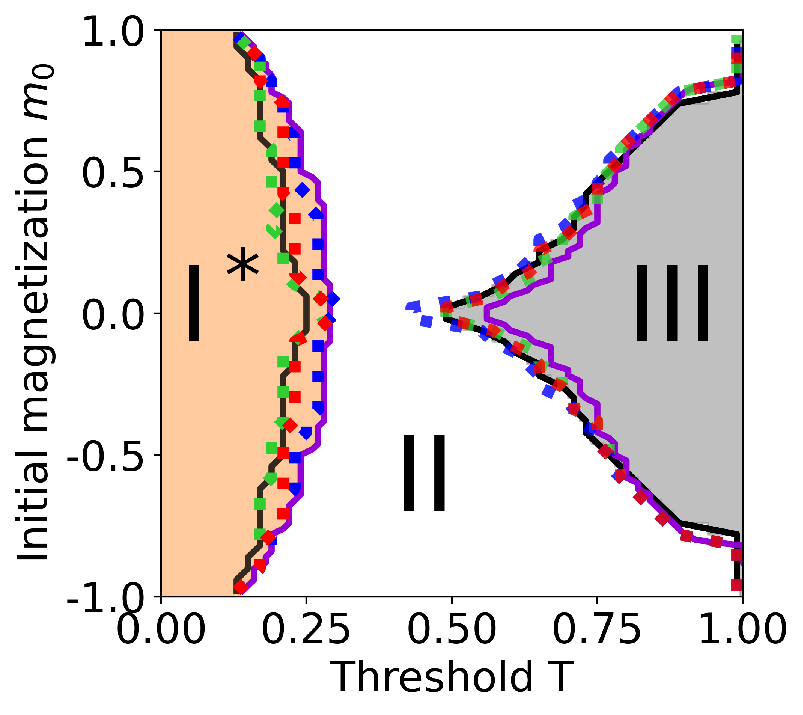
\includegraphics[width=0.5\textwidth]{Figs/Aging_STM/FIG5.pdf}
        \caption[Phase diagram modified by aging.]{\label{ER_REG_PDAGING} Phase diagram of the Symmetrical Threshold with aging model in an ER graph of $N = 4 \cdot 10^4$ nodes and $\langle k \rangle = 8$. The blue, red, and green dotted lines show the borders of Phase II (first and last value of $T$ where the system reaches the absorbing ordered state for each $m_0$) computed from numerical simulations evolving until $t_{\rm max} = 10^3$, $10^4$ and $10^5$ time steps, respectively. Black solid lines show AME solution integrated $10^5$ time steps. Phase ${\rm I}^{*}$, II and III correspond with the orange, white and gray areas, respectively. The solid purple lines are the mixed-ordered and ordered-frozen critical lines for the non-aging version of the model.}
\end{figure}

--------------------------------------------
\begin{figure}
    \centering \captionsetup{font=sf}
    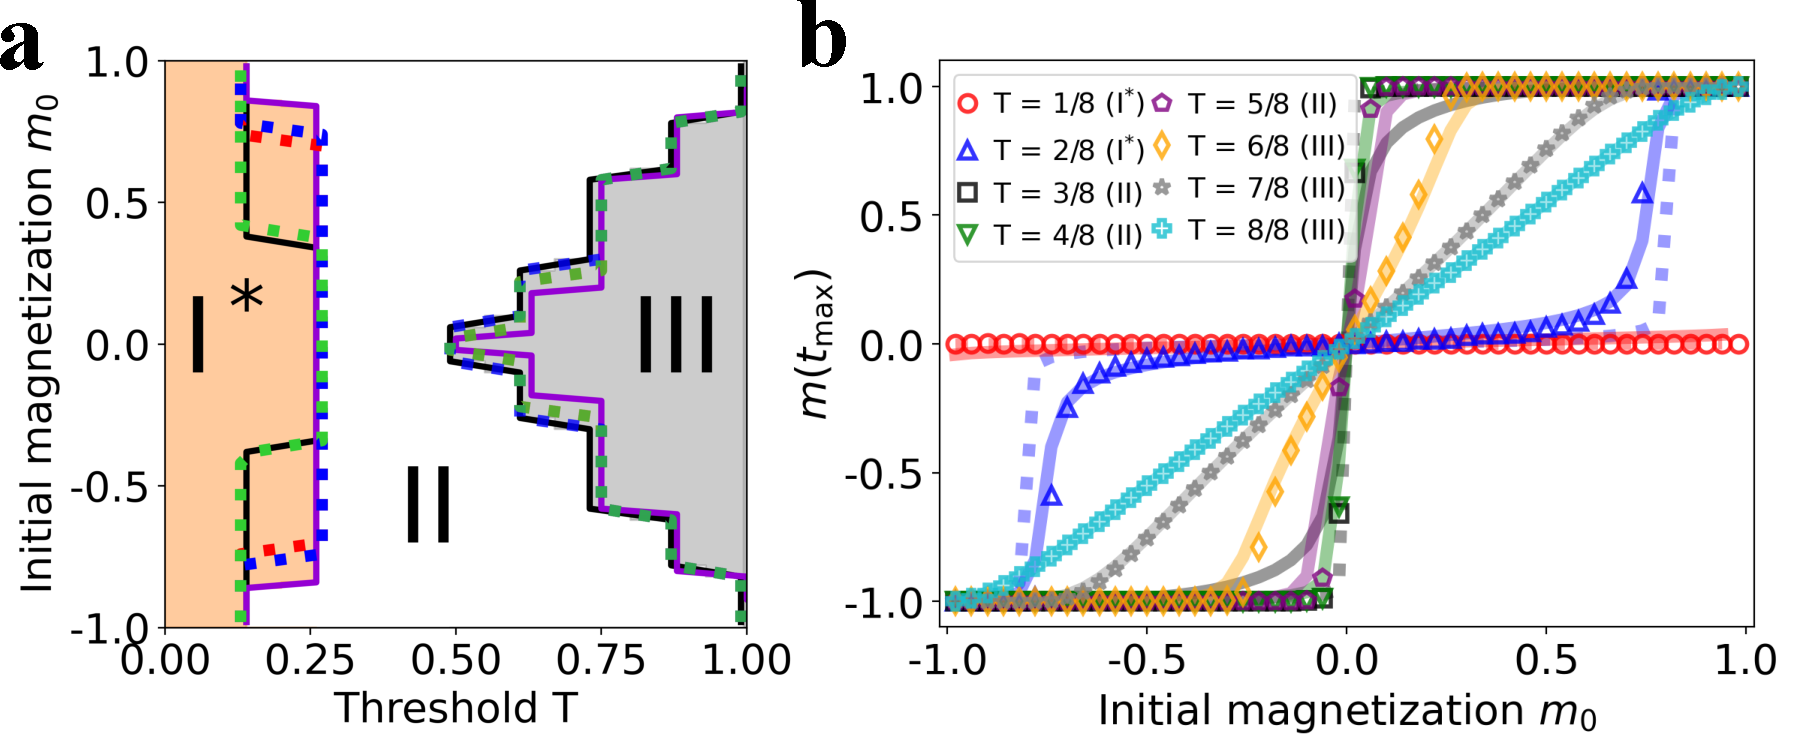
\includegraphics[width=0.85\textwidth]{Figs/Aging_STM/FIG5A.pdf}
    \caption[Symmetrical Threshold model with aging in a random regular network]{\label{REG_PDAGING} Phase diagram of the Symmetrical Threshold with aging model in a RR graph \textbf{(a)} of $N = 4 \cdot 10^4$ nodes and $\langle k \rangle = 8$. The blue, red, and green dotted lines show the borders of Phase II (first and last value of $T$ where the system reaches the absorbing ordered state for each $m_0$) computed from numerical simulations evolving until $t_{\rm max} = 10^3$, $10^4$ and $10^5$ time steps, respectively. Black solid lines show AME solution integrated $10^5$ time steps. Phase ${\rm I}^{*}$, II and III correspond with the orange, white and gray areas, respectively. The solid purple lines are the mixed-ordered and ordered-frozen critical lines for the non-aging version of the model. \textbf{(b)} Average magnetization at time $t_{\rm max}$ ($m(t_{\rm max})$) as a function of the initial magnetization $m_0$ for different values of the threshold $T$ (indicated with different colors and markers) in an 8-regular graph of $N = 4 \cdot 10^4$. Average performed over 5000 realizations evolved until $t_{\rm max} = 10^4$ time steps. Dotted and solid lines are the HMFA (for $T = 1/8 - 4/8$) and AME (for all $T$) solutions integrated numerically $10^4$ time steps.}
\end{figure}

Fig. \ref{REG_PDAGING} shows the borders of Phase II (first and last value of $T$ where the system reaches the absorbing ordered state for each $m_0$) obtained from Monte Carlo simulations running up to a maximum time $t_{\rm max}$ (dotted colored lines) for a RR graph. Reaching the stationary state in this model requires a large number of steps and it has a high computational cost. The two borders of Phase II exhibit different behavior as we increase the maximum number of time steps $t_{\rm max}$: while the ordered-frozen border does not change with different $t_{\rm max}$, the mixed-ordered border is shifted to lower values of $T$ as we increase the simulation time cutoff $t_{\rm max}$. As it occurs for the results in ER graphs (Fig. \ref{ER_REG_PDAGING}), our results suggest that Phase I is actually replaced in a good part of the phase diagram by an ordered phase in which the absorbing state $m_f = \pm 1$ is reached after a large number of time steps. The ordered-frozen border is now slightly shifted to lower values of the threshold $T$ due to aging. Figure \ref{REG_PDAGING}b shows the average magnetization on RR graphs with simulations running up to a time $t_{\rm max} = 10^4$. Upon comparison with Figure \ref{ER_REG_PD}c, the dependence on $m_0$ is quite similar, indicating the persistence of a transient mixed phase. This calls for a characterization of different phases in terms of dynamical properties and not only by the asymptotic value of the magnetization.

Regarding to the AME integrated solutions, Figure \ref{REG_PDAGING} shows the mixed-ordered and ordered-frozen transition lines predicted by the integration of the AME equations until a time cutoff $t_{\rm max}$, which show a good agreement with the numerical simulations. Figure \ref{REG_PDAGING}b also shows the predicted dependence of $m_f(m_0)$ for the RR graph. For comparison purposes, the numerical integration is computed until the highest $t_{\rm max}$ used in the Monte Carlo simulations. In addition, we apply the previously introduced HMFA to these random networks by numerically integrating Eqs. (\ref{eq:HMFaging2}). The results, displayed as dotted colored lines in Figure \ref{REG_PDAGING}b, show similarity to the AME solution for $T < 0.5$. Nevertheless, as it occurred for the HMF in the original model, this mathematical framework is not able to describe the frozen phase.


--------------------------------------------

A solution of Eq. (\ref{eq:x_f}) can be obtained numerically using standard methods, as in Ref. \cite{chen-2020}. The final magnetization is calculated as $m_f = 2 \,x_f - 1$. With this method, we obtain that the phase diagram for the model with aging is the same as for the original model (refer to Fig. \ref{COM_LAT_PD}a). As a technical point, we note that a truncation of the summation of the variable $j$ in Eq. (\ref{eq:F(A)}) is required for the numerical resolution of the implicit equation. The higher the maximum age considered $j_{\rm max}$, the higher the accuracy. With $j_{\rm max} = 5 \cdot 10^4$, the transition lines predicted by this mean-field approach show great accuracy. Moreover, by numerically integrating Eqs. (\ref{eq:HMFaging2}), the dynamical evolution of the magnetization and mean internal time can be obtained. Fig. \ref{fig:COM_AGING} shows the agreement between integrated solutions and Monte Carlo simulations of the system both for the aging and non-aging versions. It should be noted that, while aging introduces only a dynamical delay for the magnetization $m(t)$, the mean internal time $\bar{\tau}(t)$ in Phase I shows a different dynamical behavior with aging than in the original model. In this phase, due to the low value of $T$, the agents selected randomly will change their state (as they fulfill the threshold condition) and reset their internal time. Consequently, while the internal time fluctuates around a stationary value for the original model, when aging is incorporated, due to the activation probability $p_A(j)$ chosen, the mean internal time increases following a recursive relation (Eq. (\ref{eq:RR})). We refer to \ref{appendix_RR} for a derivation of this result.

\subsection{\label{sec:Complex networks aging} Random networks}

\begin{figure}
        \centering \captionsetup{font=sf}
        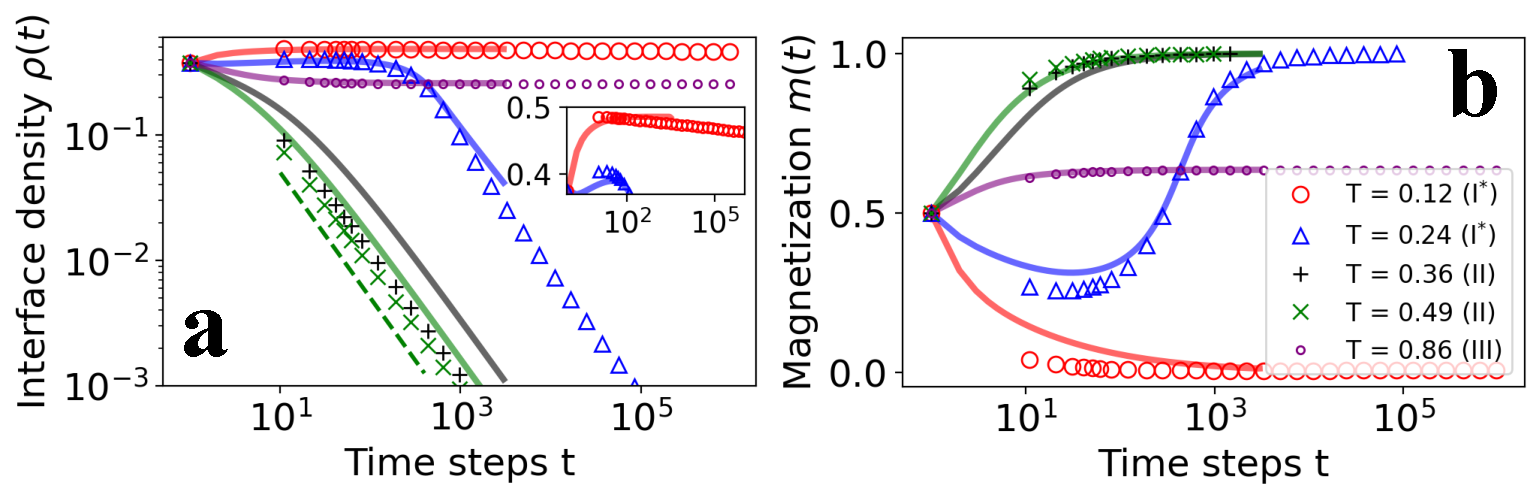
\includegraphics[width=\textwidth]{Figs/Aging_STM/FIG6.pdf}
        \caption[Symmetrical threshold model with aging dynamics in random networks]{\label{fig:evolution_random_aging} Evolution of the average interface density $\rho(t)$ \textbf{(a)} and the average magnetization $m(t)$ \textbf{(b)} for the Symmetrical Threshold model with aging. The average is computed over $5000$ surviving trajectories (simulations stop when the system reaches the absorbing ordered states) for different values of $T$, shown by different markers and colors: red ($T = 0.12$) and blue ($T = 0.24$) belong to Phase ${\rm I}^{*}$, green ($T = 0.36$) and grey ($T = 0.49$) belong to Phase II and purple ($T = 0.86$) belong to Phase III. The inset in (a) shows a close look to the evolution for $T = 0.12$, in linear-log scale. Solid colored lines are the AME integrated solutions for $10^4$ time steps, using Eqs. \ref{eq:interface} - \ref{eq:magne}. The initial magnetization is $m_0 = 0.5$. The system is on an ER graph with $N = 4 \cdot 10^4$ and mean degree $\langle k \rangle = 8$. The dashed green line in (a) shows $\rho(t) \sim \rho_0 \, t^{-1}$.
        %These expressions are written using a dimensionless time $t$. 
        As computed in Fig. \ref{fig:evolution_random}, for all $T$, $\Delta^{a}_{\rho} < 12\%$, $\Delta^{a}_{m} < 15\%$.}
\end{figure}

In contrast to the results obtained in a complete graph, aging effects have a significant impact on the phase diagram of the model on random networks. In Fig. \ref{ER_REG_PDAGING}, we show the borders of Phase II (first and last value of $T$ where the system reaches the absorbing ordered state for each $m_0$) obtained from Monte Carlo simulations running up to a maximum time $t_{\rm max}$ (dotted colored lines). Reaching the stationary state in this model requires a large number of steps (with a corresponding high computational cost). The two borders of Phase II exhibit different behavior as we increase the time cutoff $t_{\rm max}$: while the ordered-frozen border does not change with different $t_{\rm max}$, the mixed-ordered border is shifted to lower values of $T$ as we increase the time cutoff $t_{\rm max}$. Our results suggest that Phase I is actually replaced in a good part of the phase diagram by an ordered phase in which the absorbing state $m_f = \pm 1$ is reached after a large number of time steps. Similar results are found for a RR graph (see \ref{RR_phase_diagram}). The dependence of the results with $t_{\rm max}$ calls for a characterization of different phases in terms of dynamical properties rather than by the asymptotic value of the magnetization.

--------------------------------------------
\begin{figure}
    \centering \captionsetup{font=sf}
    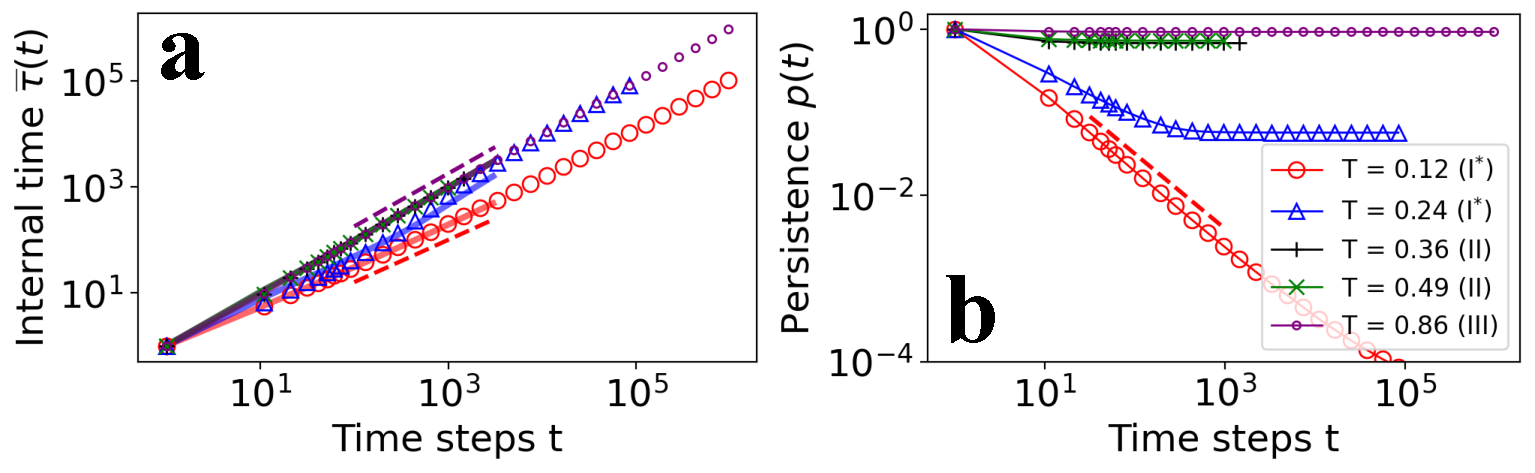
\includegraphics[width=\textwidth]{Figs/Aging_STM/FIG6A.pdf}
    \caption[Temporal dynamics of the Symmetrical threshold model with aging]{\label{fig:evolution_temporal_aging} Evolution of the mean internal time $\bar{\tau}(t)$ \textbf{(a)} and the persistence $p(t)$ \textbf{(b)} for the Symmetrical Threshold model with aging. The average is computed over $5000$ surviving trajectories (simulations stop when the system reaches the absorbing ordered states) for different values of $T$, shown by different markers and colors: red ($T = 0.12$) and blue ($T = 0.24$) belong to Phase ${\rm I}^{*}$, green ($T = 0.36$) and grey ($T = 0.49$) belong to Phase II and purple ($T = 0.86$) belong to Phase III. Solid colored lines are the AME integrated solutions for $10^4$ time steps, using Eq. \ref{eq:time}. The initial magnetization is $m_0 = 0.5$. The system is on an Erd\H{o}s-R\'enyi graph with $N = 4 \cdot 10^4$ and mean degree $\langle k \rangle = 8$. The dashed lines in (a) show $\bar{\tau}(t) = t$ (purple) and the solution from the recursive relation in Eq. (\ref{eq:RR}) (red). The dashed red line in (b) shows $p(t) = t^{-1}$. As computed in Fig. \ref{fig:evolution_random}, for all $T$, $\Delta^{a}_{\bar{\tau}} < 20\%$.}
\end{figure}

Fig. \ref{fig:evolution_temporal_aging} shows the evolution of the temporal dynamics via the mean internal time and the persistence. The persistence in Phase ${\rm I}^{*}$ shows a power-law decay, where $p(t)$ scales as $t^{-1}$, and the internal time shows an increase following the recursive relation given in Equation (\ref{eq:RR}), as it occurred for the mean-field scenario (Fig. \ref{fig:COM_AGING}). On the other hand, in Phase II, the persistence decays from $1$ to the fraction of nodes of the initial majority (the one that does not change state and reaches consensus) and the mean internal time scales linearly with time, $\bar{\tau}(t) \sim t$. For the internal time, the AME integrated solutions exhibit a remarkable concordance with the numerical simulations. Minor discrepancies between the numerical simulations and the integrated solutions can be attributed to the assumption of an infinitely sized system in the AME. As it occurred for the model without aging, the persistence cannot be predicted by this framework.
--------------------------------------------

Figure \ref{fig:evolution_random_aging} shows the time evolution of our ordering metrics. The dynamical properties are largely affected by the aging mechanism. In terms of the evolution, we find the following regimes:
\begin{itemize}
    \item \textbf{Initial mixing regime (Phase ${\rm {\bf I}}^{*}$):} It is characterized by two dynamical transient regimes: a fast initial disordering dynamics followed by a slow ordering process. After the initial fast disordering stage, the average interface density exhibits a very slow (logarithmic-like) decay. Later, due to the finite size of the system, the average interface density follows a power law decay with time, where $\rho(t)$ scales as $t^{-1}$. This phase exists for the same domain of parameters ($m_0$, $T$) as Phase I (orange region in Fig. \ref{ER_REG_PDAGING}) in the model without aging (see $T = 0.12, 0.24$ in Fig. \ref{fig:evolution_random_aging});
    \item \textbf{Ordered regime (Phase II):} According to the initial majority, the magnetization tends to the ordered absorbing state. This regime is characterized by a power-law interface decay, where $\rho(t)$ scales as $t^{-1}$. (see $T = 0.36, 0.49$ in Fig. \ref{fig:evolution_random_aging});
    \item \textbf{Frozen regime (Phase III):} Each individual realization is characterized by an initial tendency towards the majority consensus, but very fast reaches an absorbing frozen configuration (see $T = 0.86$ in Fig. \ref{fig:evolution_random_aging}).
\end{itemize}
The main effect of aging is that the mixed states of Phase I are no longer present, at least not for the type of networks that we are analyzing here. We will show later that Phase I reemerges in denser graphs. Instead, for sparse graphs, we observe a new Phase ${\rm I}^{*}$ in which the system initially disorders and later orders until reaching the absorbing states $m_f = \pm 1$. This behavior is shown in Fig. \ref{fig:evolution_random_aging} for $T = 0.12$ and $0.26$. For $T = 0.12$, the system initially disorders, and then the interface density follows a logarithmic-like decay (see inset in Fig. \ref{fig:evolution_random_aging}a). Due to the slow decay, the system stays in this transient regime even after $10^{6}$ time steps, and the fall to the absorbing states is not observed in this figure. Similarly, for $T = 0.26$ the disordering process stops and then the system gradually evolves towards a fully ordered state. For this value of $T$, the logarithmic-like decay is not appreciated and we just observe the power-law decay due to the finite size of the system. The difference between $T = 0.12$ and $T = 0.26$ comes from the fact that in this Phase ${\rm I}^{*}$, the interface decay becomes faster as we increase the threshold $T$ (see Fig. \ref{fig:mixed_phase}(a-c)). Notice the different interface decay in Fig. \ref{fig:mixed_phase}c (inset) between values of $T < 0.3$ (Phase ${\rm I}^{*}$), where all trajectories show a logarithmic-like decay of $\rho(t)$ in a transient regime, and $T \geq 0.3$ (Phase II), where trajectories from the initial condition exhibit fast ordering dynamics towards the majority consensus. Moreover, we observe that in Phase ${\rm I}^{*}$, the initial magnetization $m_0$ introduces a bias to the stochastic process, implying that the larger $m_0$ in absolute value, the larger the number of realizations that reach the absorbing state with the same sign of $m_0$. However, the system can still reach the absorbing state of the opposite sign of $m_0$ (initial minority), as shown in the trajectories with $T = 0.25$ in Fig. \ref{fig:mixed_phase}a. Due to the characteristic logarithmic decay of Phase ${\rm I}^{*}$, a statistical analysis of the inversion process incurs a significant computational cost. In Fig. \ref{fig:mixed_phase}b, we present the final magnetization histogram for $T=0.25$, a value proximal to the ${\rm I}^{*} - {\rm II}$ boundary where this analysis is computationally feasible. As depicted in this figure, the proportion of realizations in which consensus is reached in the initial minority state is approximately $3.3\%$.

\begin{figure}
    \centering \captionsetup{font=sf}
    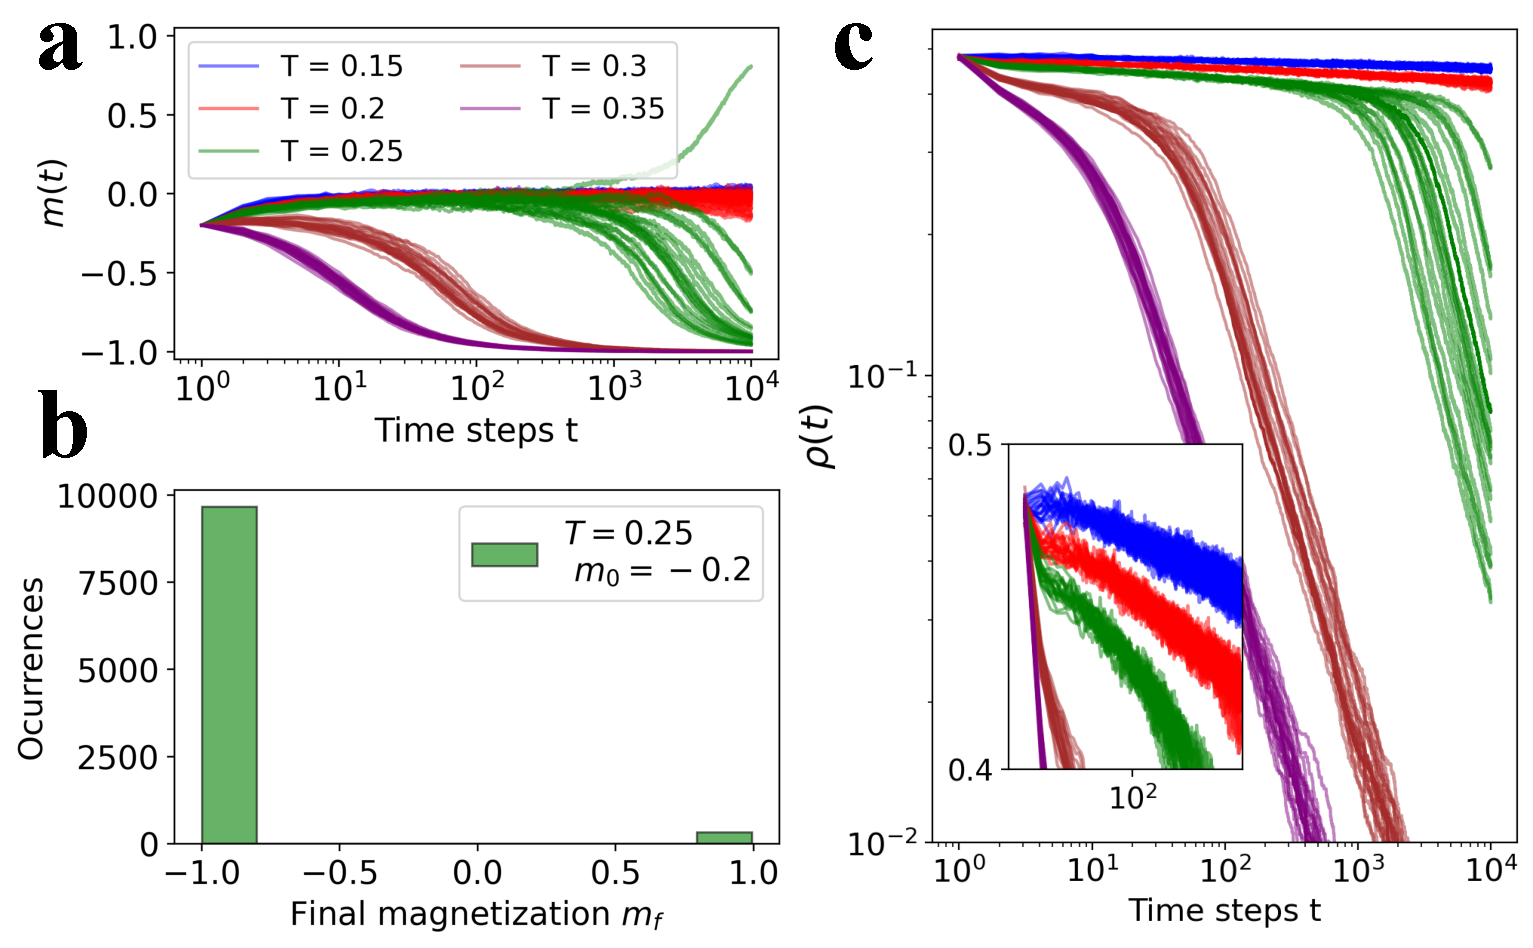
\includegraphics[width=0.9\textwidth]{Figs/Aging_STM/FIG7.pdf}
    \caption[Phase ${\rm I}^{*}$ slow decay and minority consensus]{\label{fig:mixed_phase} Magnetization $m(t)$ \textbf{(a)} and interface density $\rho(t)$ \textbf{(c)} trajectories for different values of the threshold $T$ ($m_0 = -0.2$) using the Symmetrical Threshold model with aging. \textbf{(b)} Final magnetization histogram of $1000$ trajectories for the same system at $T=0.25$. Different colors indicate different values of $T$. The inset at (b) shows a close look at the logarithmic-like decay, shown in linear-log scale. The system is an ER graph with $N = 4 \cdot 10^4$ and mean degree $\langle k \rangle = 8$.}
\end{figure}
In Phase II, the system asymptotically orders for any initial condition as in the original model, but the dynamical properties are modified due to the presence of aging: the exponential decay of the interface density is replaced by a slow power-law decay, where the exponents of the exponential and the power-law are found to be similar. Contrary, the dynamical properties of Phase III are not affected by the presence of aging. The temporal magnitudes analysis (mean internal time and persistence) can be found in \ref{sec:temporal_dynamics}. 

As it occurred for the non-aging version of the model, the dynamical characterization discussed above holds for all possible
$m_0$ except for the symmetric initial condition $m_0 = 0$. The implications of the order-disorder transition (that occurs at a critical mean degree $k_c (N)$) \cite{Konstantin} are still present in the model with aging.

To account for the results of our Monte Carlo simulations, we use the same mathematical framework as described in Equation (\ref{eq:AME_age}). According to the update rules of the Symmetrical Threshold Model with aging, the transition probabilities now depend on the age $j$, as given by the activation probability  $p_A (j)$:
\begin{eqnarray}
    &T^{+}_{k,m,j} = p_A(j) \, \theta(m/k - T) \quad \quad T^{-}_{k,m,j} = p_A(j) \, \theta((k-m)/k - T), \nonumber\\
    &A^{\pm}_{k,m,j} = 1 - T^{\pm}_{k,m,j}.
\end{eqnarray}
We show in Figure \ref{ER_REG_PDAGING} the mixed-ordered and ordered-frozen transition lines predicted by the integration of the AME equations until a time cutoff $t_{\rm max}$. We find good agreement between the theoretical predictions and the simulations both for ER and RR networks (see RR results in \ref{RR_phase_diagram}). Regarding dynamical properties, the AME integrated solutions exhibit a remarkable concordance with the evolution of all the metrics as shown in Figure \ref{fig:evolution_random_aging}. Minor discrepancies between the numerical simulations and the integrated solutions are attributed to the different assumptions, discussed previously, on which the AME is based.  
\begin{figure}
        \centering \captionsetup{font=sf}
        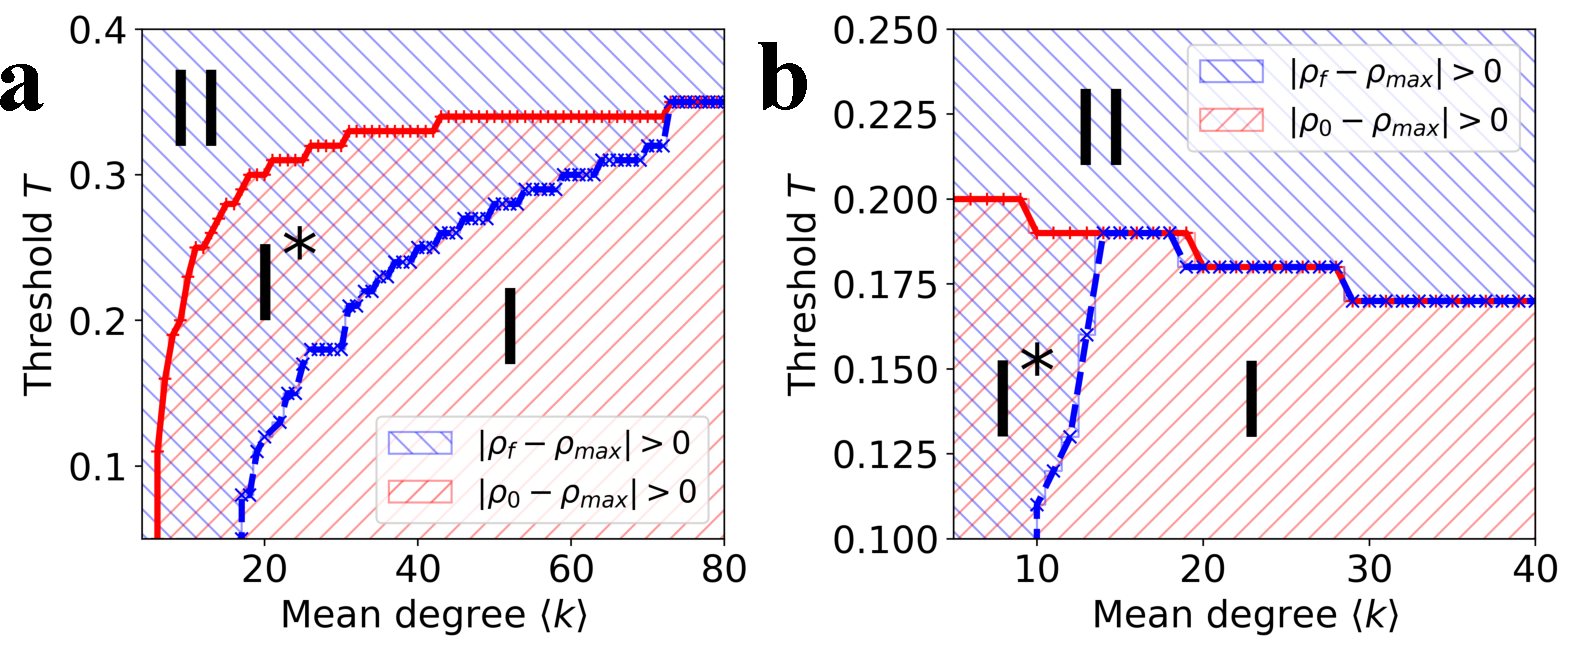
\includegraphics[width=0.95\textwidth]{Figs/Aging_STM/FIG8.pdf}
        \caption[Phase ${\rm I}^{*}$ dependence with the network mean degree]{\label{fig:PD_Z} Critical threshold $T_c$ dependence with the mean degree $\langle k \rangle$ for the Symmetrical Threshold model with aging for an ER graph with $N = 4 \times 10^4$ nodes for an initial magnetization of $m_0 = 0.25$ \textbf{(a)} and $m_0 = 0.75$ \textbf{(b)}. The blue and red markers indicate the borders of phases I and II, which coincide for a sufficiently large value of the mean degree. The hatched area corresponds to the fulfillment of the inequality in the legend.}
\end{figure}

The numerical results discussed so far are for random networks with average degree $\langle k \rangle = 8$. According to them and to the analytical insights, one can conclude that aging significantly changes the phase diagram for sparse networks. However, we know that the model with aging shows the same phase diagram as the model without aging for a fully connected network. This implies that, for ER graphs, as the mean degree $\langle k \rangle$ approaches $N$, Phase ${\rm I}^{*}$ must disappear. Therefore, the combined effects of increasing the mean degree and introducing aging need to be investigated in more detail. Phase II is distinguishable from phases I and ${\rm I}^{*}$ because the system initially orders, i.e., $|\rho_0 - \rho_{\rm max}| = 0$, where $\rho_{\rm max}$ is the maximum value attained by the interface density during the dynamical evolution. In contrast, Phase I is distinguished from Phases ${\rm I}^{*}$ and II because the system remains disordered, i.e., $|\rho_{\rm max} - \rho(t_{\rm max})| \approx 0$. Thus, Phase ${\rm I}^{*}$ is the only phase among these three where $|\rho_0 - \rho_{\rm max}| > 0$ and $|\rho_{\rm max} - \rho(t_{\rm max})| > 0$. Using this criterion, we studied the dependence of the critical threshold  $T_c$ on the mean network degree defining the transition lines between phases I, ${\rm I}^{*}$, and II (see Fig. \ref{fig:PD_Z}). In the absence of aging, the red line in Fig. \ref{fig:PD_Z} gives the value of the mixed-ordered transition line $T_c$. When aging is included, at low degree values, Phase I is replaced by ${\rm I}^{*}$, as expected. However, as the mean degree increases, Phase I emerges despite the presence of aging, leading to the coexistence of phases I and ${\rm I}^{*}$ in the same phase diagram over a range of mean degree values. As the mean degree is further increased, a critical value is reached where Phase ${\rm I}^{*}$ is no longer present, and the discontinuous transition I-II occurs at the same value than in the model without aging. Importantly, this critical mean degree at which Phase ${\rm I}^{*}$ disappears, depends significantly on the initial magnetization $m_0$.

\section{\label{sec: Dynamics on a Moore Lattice}  Dynamics on a Moore Lattice}

\subsection{The role of aging}

\begin{figure}
        \centering \captionsetup{font=sf}
        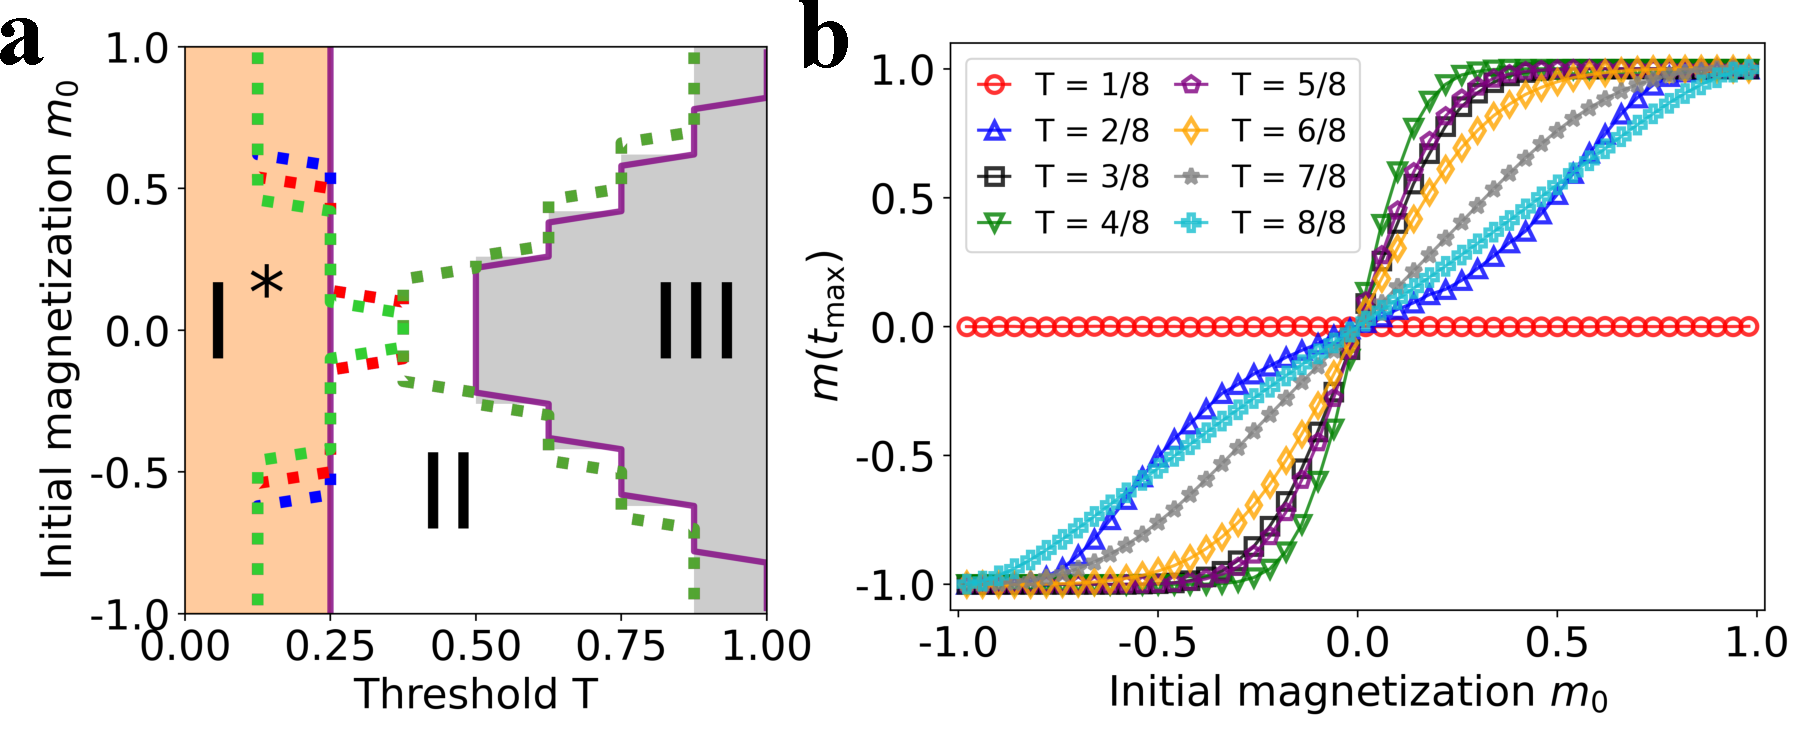
\includegraphics[width=\textwidth]{Figs/Aging_STM/FIG11.pdf}
        \caption[Symmetrical Threshold model with aging in a Moore lattice]{\label{LAT_PDAGING} \textbf{(a)} Phase diagram of the Symmetrical Threshold model with aging in a Moore lattice of $N = L \times L$, with $L = 100$. The blue, red and green dotted lines show the borders of Phase II (first and last value of $T$ where the system reaches the absorbing ordered state for each $m_0$) from numerical simulations evolving until $t_{\rm max} = 10^3$, $10^4$ and $10^5$ time steps, respectively. Phase ${\rm I}^{*}$, II and III correspond with the orange, white and gray areas, respectively. The solid purple lines are the mixed-ordered and ordered-frozen critical lines for the Symmetrical threshold model (from Fig. \ref{LAT_PD}). \textbf{(b)} Average magnetization at time $t_{\rm max}$ ($m_f(t_{\rm max})$) as a function of the initial magnetization $m_0$ for different values of the threshold $T$ (indicated with different colors and markers) in a Moore lattice of $N = L \times L$, with $L = 100$. The numerical simulations are obtained until $t_{\rm max} = 10^4$ time steps. Average performed over 5000 realizations.}
\end{figure}

We show in Figure \ref{LAT_PDAGING}a the borders of Phase II obtained from numerical simulations running up to a time $t_{\rm max}$ (dotted colored lines). Similarly to the behavior observed in random networks, the mixed-ordered border is shifted to lower values of $T$ as we increase the simulation time cutoff $t_{\rm max}$. Thus, Phase I is replaced by an ordered phase due to the aging mechanism. Examining the dependence of the final value of the magnetization on its initial condition  $m_f(m_0)$  (Figure \ref{LAT_PDAGING}b), one can conclude that the mixed phase is still present, at least transiently, as in the initial disordering phase described in the previous section (Phase ${\rm I}^{*}$). Phase II is again characterized by an asymptotically ordered state where the initial majority reaches consensus. However, for this specific structure, near $m_0 = 0$ and $T = 1/2$, the ordered state is not reached for any threshold value. Furthermore, comparing with Fig. \ref{LAT_PDAGING}b with the results from the model without aging (Fig. \ref{LAT_PD}b), the discontinuous jump at $m_0 = 0$ for $T = 3/8, 4/8$ is replaced by a continuous transition, where a range of states with $0 < |m_f| < 1$ are present around $m_0 = 0$. To determine whether these states belong to Phase ${\rm I}^{*}$, II or III, we need again a characterization of phases in terms of dynamical properties. According to the results in Figure \ref{fig:evolution_lattice_aging}, we find here the same regimes identified for random networks:
\begin{itemize}
    \item \textbf{Initial mixing regime (Phase ${\rm {\bf I}}^{*}$):}  After the initial disordering stage, the average interface density shows a very slow decay reflecting the slow growth of spatial domains in each binary state. The persistence in this phase shows a power-law decay $p(t) \sim t^{-1}$ (see $T = 1/8,2/8$ in Fig. \ref{fig:evolution_lattice_aging});
    \item \textbf{Ordered regime (Phase II):} It is characterized by coarsening dynamics that end in the absorbing states $m_f = \pm 1$. The form of the decay of the interface density depends on the value of $m_0$ (see $T = 3/8,4/8$ in Fig. \ref{fig:evolution_lattice_aging});
    \item \textbf{Frozen regime (Phase III):} It is characterized by an initial tendency to order but the system very fast reaches an absorbing frozen configuration (see $T = 5/8,7/8$ in Fig. \ref{fig:evolution_lattice_aging}).
\end{itemize}

\begin{figure}
        \centering \captionsetup{font=sf}
        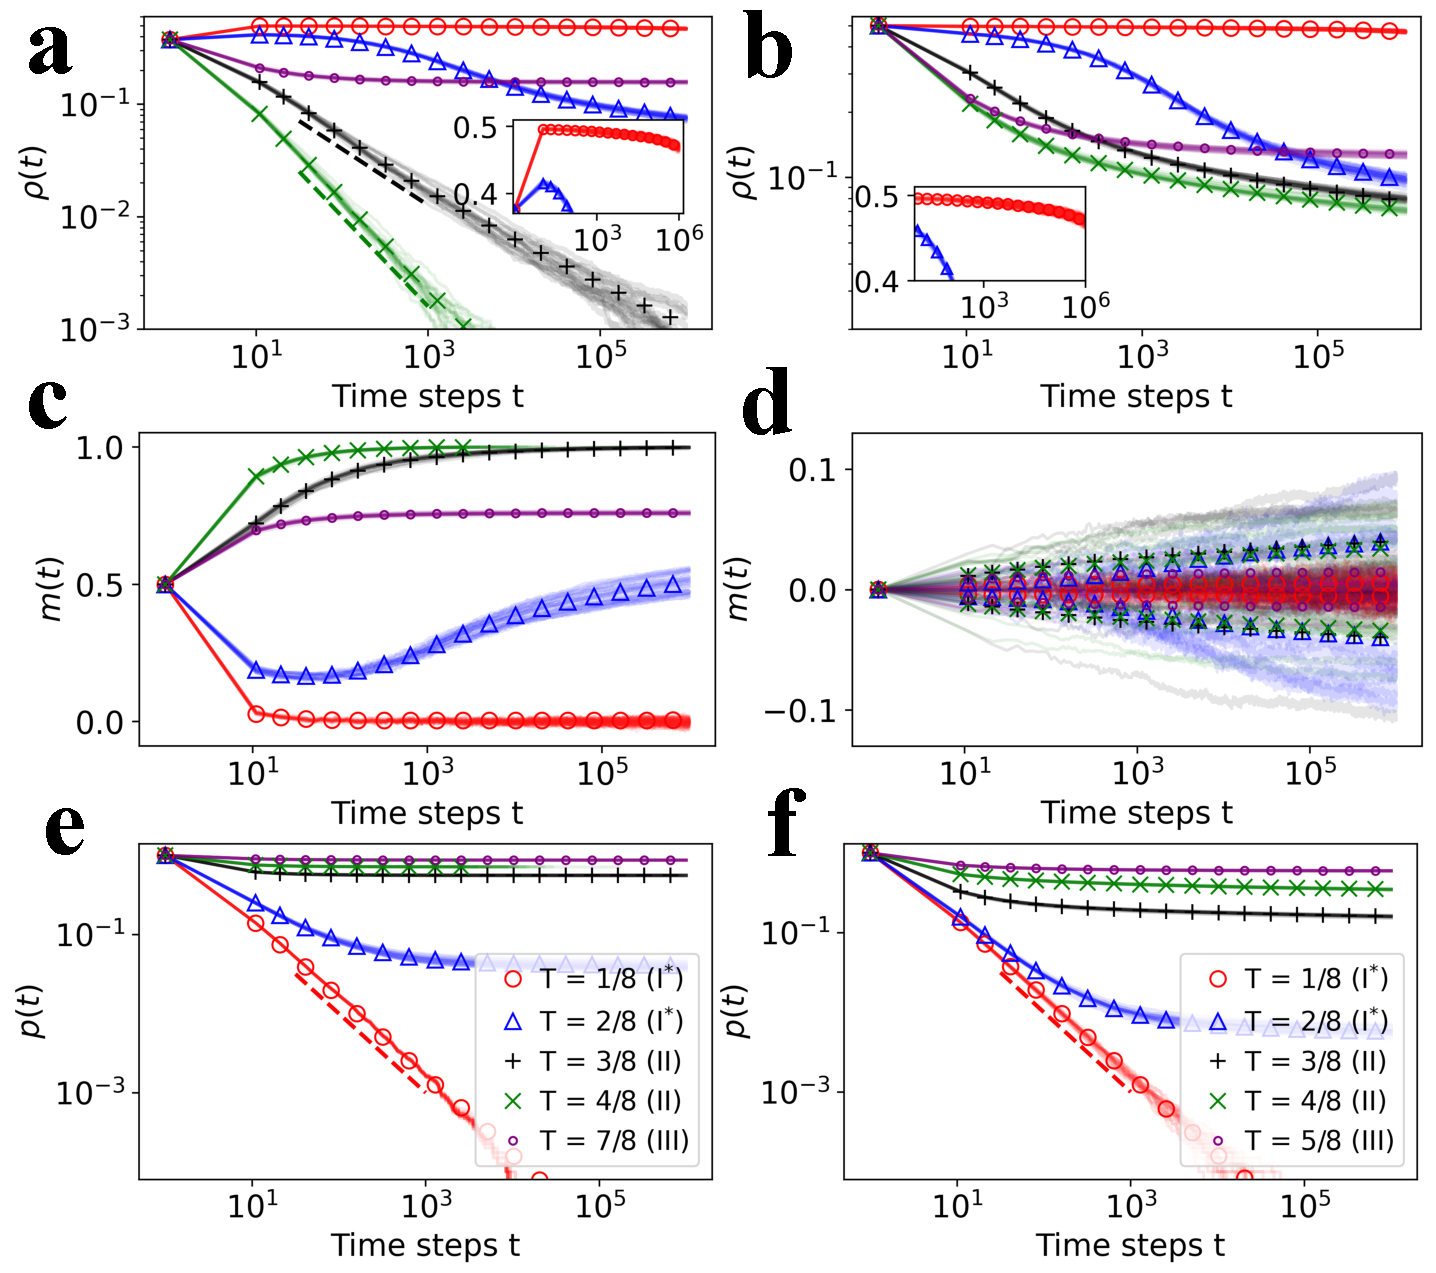
\includegraphics[width=\linewidth]{Figs/Aging_STM/FIG12.pdf}
        \caption[Modified dynamical regimes by aging in a Moore lattice]{\label{fig:evolution_lattice_aging} Evolution of the average interface density $\rho(t)$ \textbf{(a-b)}, the average magnetization $m(t)$ \textbf{(c-d)}, and the persistence $p(t)$ \textbf{(e-f)} for the Symmetrical model with aging in a Moore lattice starting from a random configuration with $m_0 = 0.5$ (a-c-e) and $m_0 = 0$ (b-d-f). We plot 30 different trajectories in solid lines and the average of over $5000$ surviving trajectories in symbols. Colors and symbols indicate different threshold values: red ($T = 1/8$) and blue ($T = 2/8)$ belong to Phase ${\rm I}^{*}$, green ($T = 3/8$), and black ($T=4/8$) belong to Phase II, and purple ($T = 5/8, 7/8$) belong to Phase III. The average magnetization is computed according to the two symmetric absorbing states. The insets in (a-b) show a close look at the evolution for $T = 0.12$, in linear-log scale. System size is fixed at $N = L \times L$, $L = 200$. The dashed lines in (a) are $\rho \sim t^{-\alpha}$ with $\alpha = 0.5$ (black) and $\alpha = 0.8$ (green), and in (c) are $p(t) \sim t^{-1}$ (red). 
        %These expressions are written using a dimensionless time $t$.
        Simulations stop when the system reaches the absorbing ordered states.}
\end{figure}

The implications of aging become explicit by comparing the dynamical properties of the cases with aging (Figure \ref{fig:evolution_lattice_aging}) and without aging (Figure \ref{fig:evolution_lattice}). When the threshold is $T<3/8$, Phase ${\rm I}$ is replaced by Phase ${\rm I}^{*}$ in which there is an initial disordering process very fast followed by a slow coarsening process that accelerates when we increase the threshold. Although the aging implications in this phase are similar to those observed in the ER graph, the coarsening process is slower  (see insets in Fig. \ref{fig:evolution_lattice_aging}a-b).

In Phase II ($T=3/8, 4/8$) and when $m_0=0.5$, the system exhibits coarsening towards the ordered state $m_f=\pm 1$. In this case, the interface decay $\rho \sim \exp(-\alpha \, t)$, observed in the absence of aging is replaced, due to aging, by a power law decay $\rho \sim t^{-\alpha}$, as noted in Ref. \cite{Abella-2022-AME}. We find $\alpha=0.5$ and $0.8$ for $T=3/8$ and $4/8$, respectively. For $m_0=0$, the power law decay of the interface density vanishes with aging, and the system exhibits coarsening dynamics much slower than for an unbalanced initial condition. In this region of the phase diagram, spatial clusters start to grow from the initial condition, but once formed, it takes a long time for the system to reach the absorbing state $m_f = \pm 1$. 
%In this region, aging prevents the small clusters from disintegrating but also keeps the system away from reaching the absorbing ordered state. 
We note that for these parameter values, the system is not able to reach $|m|$ over $0.1$ even after $10^6$ time steps, but since there is coarsening from the initial condition, the expected stationary state as $t \to \infty$ is $m_f=\pm1$. There is neither initial disordering nor freezing, these values correspond to the defined Phase II, even though the system exhibits ``long-lived segregation'' long transient dynamics (see the difference with the dynamics of the model without aging in Fig. \ref{fig:snapshots}). In Fig. \ref{LAT_PDAGING}a, we differentiate Phase II from Phase III by analyzing the activity in the system: If agents are changing, even though the interface decay is slow, the system is in Phase II. If agents are frozen, it lies in Phase III. When comparing the ordered-frozen critical line to the one from the original model (purple line), we notice that aging causes certain values ($m_0$, $T$) that were previously in Phase II near the critical line to enter the frozen phase.

\begin{figure}
        \centering \captionsetup{font=sf}
        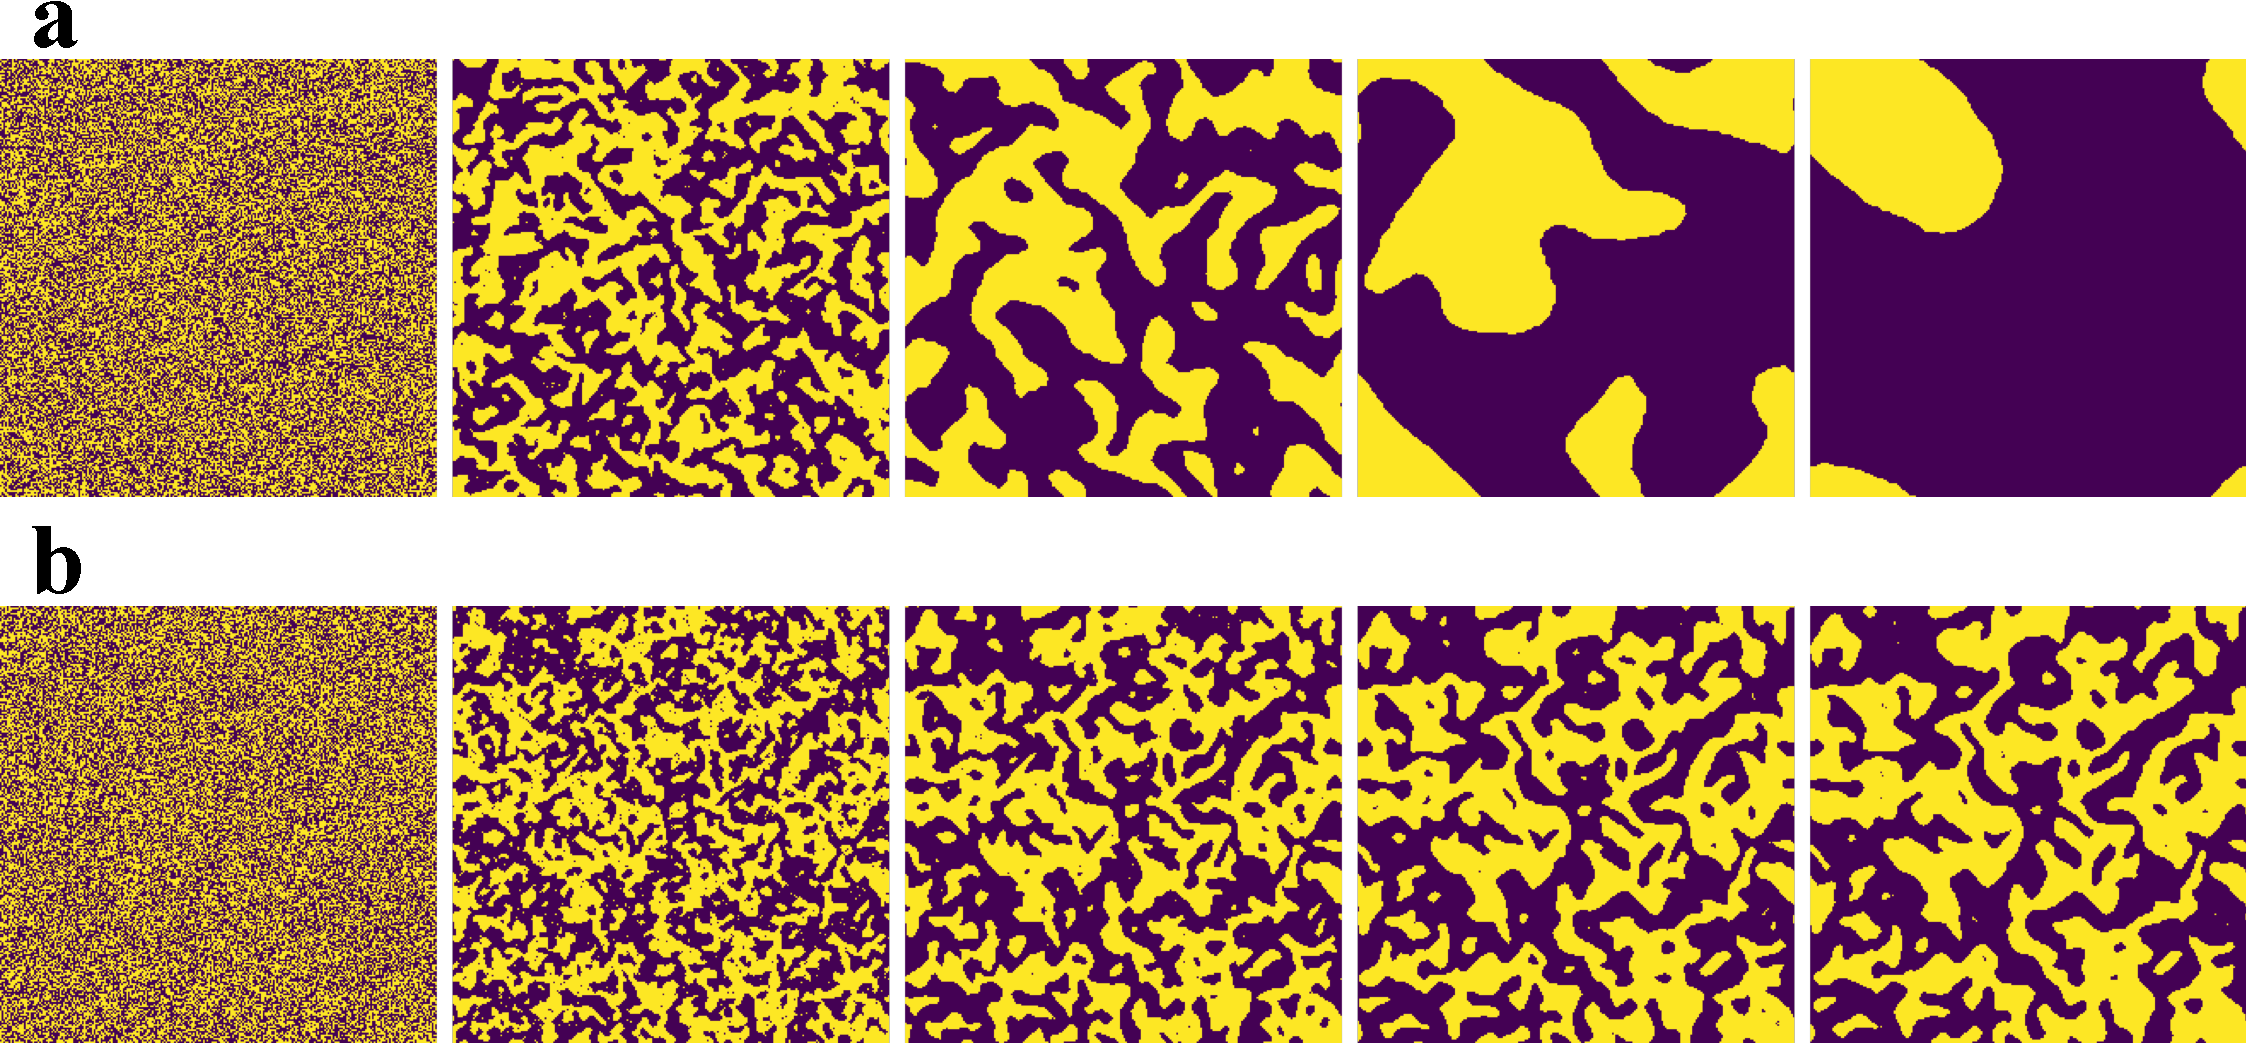
\includegraphics[width=\linewidth]{Figs/Aging_STM/FIG13.pdf}
        \caption[System evolution at $T = 0.5$ and $m_0 = 0$]{\label{fig:snapshots} Evolution of a single realization for $T = 0.5$ and $m_0 = 0$ using the Symmetrical threshold model \textbf{(a)} and the version with aging \textbf{(b)}. Snapshots are taken after $1,10,60,440$ and $3300$ time steps in (a) and after $1,60,3300,2 \cdot 10^5$ and $5 \cdot 10^6$ time steps in (b), increasing from left to right. System size is fixed to $N = L \times L$, $L = 256$.}
\end{figure}

Finally, it should be noted that in Phase ${\rm I}^{*}$, the initial disordering dynamics drive the system towards $m=0$. Therefore, the subsequent coarsening dynamics follow the slow interface decay observed in Phase II for $m_0 \sim 0$. Thus, the presence of aging implies that the system asymptotically orders for any initial condition, but due to the initial disordering, the coarsening dynamics fall into the ``long-lived segregation'' regime independently of the initial condition. 

%Aging prevents the small clusters to be disintegrated, which leads to order from a mixed state but slows down the coarsening process. In Fig. \ref{fig:snapshots_model_aging} we show a single trajectory evolution for $T = 0.5$ where, even after $5 \cdot 10^6$ time steps, there are several clusters in the system and no clear majority (long-lived segregation). If our initial condition has a sufficiently large initial bias $|m_0| > 0$, the fully ordered state $m_f = \pm 1$ is reached (as observed in Fig. \ref{COM_LAT_PDAGING}b), following a persistence and interface decay proportional to the activation probability $p_A(t)$. Regarding the frozen phase, the dynamics are similar to the original model, but aging prevents the system from freezing fast and there is activity in the system even after $10^5$ time steps.The new ordered phase does not exhibit the same dynamics for all values of $T$ and $m_0$, but the final state is the same: one absorbing state $m_f = \pm 1$. Keeping $T = 0.25$ constant, Fig. \ref{fig:mixed_ro_LAT} shows that there are several values of $m_0$ for which the system initially tends to $m = 0$ but, at a certain moment, aging starts to be relevant and leads the system to order. The interface density $\rho(t)$ shows a similar dependency regardless of $m_0$. Notice that, for $m_0 = -0.1$, the system has an initial majority, but there are realizations ordering towards both absorbing states $m_f = \pm 1$. Therefore, as an effect of aging, an initial minority is able to reach consensus in this region of the phase diagram. Fig.\ref{fig:snapshots_mixed} shows a typical realization in a Moore lattice to show the domain growth. Initially, the system is dominated by the yellow opinion but, after some time steps, it tends towards a mixed state where domains start to grow for both opinions until there is a majority of yellow opinion that dominates. It is counterintuitive that, including aging as the memory of the time steps in the current state, the system is able to "forget" the initial state and reaching consensus becomes a stochastic process. On the other hand, keeping $m_0$ constant and increasing $T$ leads the system to a faster interface decay (see Fig. \ref{fig:mixed_t_LAT}).


%ordered transition shows now an apparent dependence on $m_0$ as a result of aging. In Fig. \ref{fig:mf_variar_T_lat}, the model with aging reaches an ordered state for several values where the original model exhibited a mixed phase for $T = 0.24$. Moreover, Fig. \ref{fig:mf_variar_tmax_lat} shows that the system tends to order as we increase $t_{\rm max}$. The same would occur for $T = 0.12$ if we wait a larger number of time steps (as it is shown when we analyze the dynamics). Therefore, the full mixed phase is replaced by a new ordered phase due to the aging effects. On the other hand, for large values of $T$, the frozen phase shows a similar dependence of the final state with $m_0$ to the original model. In addition, for the values where the ordered phase was exhibited in the original model ($T = 3/8,4/8$), the aging modifies the phase diagram close to $m_0 = 0$. Comparing with Fig. \ref{fig:lattice}, a range of stationary states with $0 < |m_f| < 1$ appear around $m_0 = 0$. These are states of the system where both opinions coexist for a very long time. One may think that these states belong to the frozen phase, but the final state is dynamically active (see the tendency to order in Fig. \ref{fig:mf_variar_tmax_lat}). Thus, due to a stochastic effect, the system may fall to the absorbing state but the time to reach the absorbing state is very large even for small system sizes. We name this region of the phase diagram as "long-lived segregation", which occurs at $T < 0.5$ close to $m_0 = 0$.

\section{\label{sec:Summary and Conclusions} Summary and discussion}


In this work, we have studied with Monte Carlo numerical simulations and analytical calculations the Symmetrical Threshold Model. In this model, the agents, nodes of a contact  network, can be in one of the two symmetric states $\pm 1$.  System dynamics follows a complex contagion process in which a node changes state when the fraction of neighboring nodes in the opposite state is above a given threshold $T$. For $T=1/2$, the model reduces to a majority rule or the zero temperature Spin Flip Kinetic Ising Model. When the change of state is only possible in one direction, say from $1$ to $-1$, it reduces to the Granovetter-Watts Threshold model \cite{granovetter-1978,watts-2002,Abella-2022-AME}. We have considered the cases of a fully connected network, Erd\H{o}s-Rényi, and random regular networks, as well as a regular two-dimensional Moore lattice. 

We have found that, in the parameter space of threshold $T$ and initial magnetization $m_0$, the model exhibits three distinct phases, namely Phase ${\rm I}$ or mixed, Phase ${\rm II}$ or ordered, and Phase ${\rm III}$ or frozen. The existence of these three phases is robust for different network structures.
% and the mixed-ordered and ordered-frozen transitions show nontrivial dependence on the threshold and the initial magnetization ($T_{c}(m_0)$ and $T_{c}^{*}$). 
These phases are well characterized by the final state ($m_f$), and by dynamical properties such as the interface density $\rho(t)$, time-dependent average magnetization $m(t)$, persistence times $p(t)$, and mean internal time $\bar{\tau}(t)$. These phases can be obtained analytically in the mean-field case of a fully connected network. For the random networks considered, we derive an approximate master equation (AME) \cite{gleeson-2013,Abella-2022-AME} considering agents in each state according to their degree $k$,  neighbors in state $-1$, $m$, and age $j$. From this AME, we have also derived a heterogeneous mean-field (HMF) approximation. While the AME reproduces with great accuracy the results of Monte Carlo numerical simulations of the model (both static and dynamic), the HMF shows an important lack of agreement, highlighting the importance of high-accuracy methods necessary for threshold models. 

%For the random networks studied, we derived a mathematical description based on approximate master equation and am heterogeneous mean-field approximation. We found that, as it occurred for the Watts' threshold model, the HMF approximation is not enough to describe the full phase diagram, even though it captures qualitatively the mixed-ordered transition. On the other hand, the full AME gives a good description of the full phase diagram for the networks studied here, even though it has a high computational cost. Regarding the dynamics, from our AME numerical solution we extracted the information about the magnetization, the interface density and the persistence. While for $m(t)$ and $p(t)$ the AME matches the numerical simulations with great accuracy, for $p(t)$ the AME description does not match the results from numerical simulations. We associate this error to the finite size effects, which are more relevant for this magnitude.

%Aging is incorporated as a resistance to state change that is inversely proportional to the persistence time.
Aging is incorporated in the model as a decreasing probability to modify the state as the time already spent by the agent in that state increases. The key finding is that the mixed phase (Phase ${\rm I}$), characterized by an asymptotically disordered dynamically active state, does not always exist: the aging mechanism can drive the system to an asymptotic absorbing ordered state, regardless of how low the threshold $T$ is set. A similar effect of aging was already described for the Schelling model in Ref. \cite{Abella-2022}. When the dynamics are examined in detail, a new Phase ${\rm I}^{*}$, defined in terms of dynamical properties, emerges in the domain of parameters where the model without aging displays Phase ${\rm I}$. This phase is characterized by an initial disordering regime ($m \to 0$) followed by a slow ordering dynamics, driving the system toward the ordered absorbing states (including the one with spins opposite to the majoritarian initial option). This result is counter-intuitive since aging incorporates memory into the system, yet in this phase, the system ``forgets'' its initial state. The network structure plays an important role in the emergence of Phase ${\rm I}^{*}$ since it does not exist for complete graphs. A detailed analysis reveals that Phase ${\rm I}^{*}$ replaces Phase ${\rm I}$ only for sparse networks, including the case of the Moore lattice. For ER networks we find that, as the mean degree increases, Phase ${\rm I}$ reappears and there is a range of values of the mean degree for which phases ${\rm I}$ and ${\rm I}^{*}$ coexist. Beyond a critical value of the mean degree, Phase ${\rm I}$ extends over the entire domain of parameters where Phase ${\rm I}^{*}$ was observed.

While aging favors reaching an asymptotic absorbing ordered state for low values of $T$ (Phase ${\rm I}$), in Phase II the ordering dynamics are slowed down by aging, changing, both in random networks and in the Moore lattice, the exponential decay of the interface density by a power law decay with the same exponent. The aging mechanism is found not to be important in the frozen Phase ${\rm III}$. All these effects of aging in the three phases are well reproduced for random networks by the AME derived in this work, which is general for any chosen activation probability $p_A (j)$.

For the Moore lattice, we have also considered in detail the special case of the initial condition $m_0=0$. In this case, Phase ${\rm I}^{*}$ emerges, and Phase ${\rm III}$ is robust against aging effects. However, in Phase ${\rm II}$ aging destroys the characteristic power law decay of the interface density, $\rho(t) \sim at^{-1/2}$, associated with curvature reduction of domain walls. This would be a main effect of aging in the dynamics of the phase transition for the zero temperature spin flip Kinetic Ising model \cite{gunton1983}. Additionally, this regular structure allowed us to analyze the effects of a compact initial condition. We have shown that the joint effect of aging and a compact initial condition prevent the ordered phases from reaching the consensus state (see \ref{sec:compact_condition}).

As a final remark on the general effects of aging in different models of collective behavior, we note that the replacement of a dynamically active disordered stationary phase by a dynamically ordering phase is generic. In this paper, we find the replacement of Phase ${\rm I}$ by Phase ${\rm I}^{*}$. Likewise in the Voter model, aging destroys long-lived dynamically active states characterized by a constant value of the average interface density, and it gives rise to coarsening dynamics with a power law decay of the average interface density \cite{fernandez-gracia-2011}. In the same way, in the Schelling segregation model, a dynamically active mixed phase is replaced, due to the aging effect, by an ordering phase with segregation in two main clusters. 
Another aging effect that seems generic, in phases in which the system orders when there is no aging, is the replacement of dynamical exponential laws by power laws. This is what happens here in  Phase ${\rm II}$ for the decay of the average interface density but, likewise, exponential cascades in the Granovetter-Watts model are replaced due to aging by a power-law growth with the same exponent \cite{Abella-2022-AME}.

Further research with the general AME used in this study would involve a new approach that considers the master equation, as described in Ref. \cite{peralta-2020B}. This approach aims to incorporate finite size effects, which are relevant when $m_0$ is close to zero, and would provide a mathematical framework for further analyisis of the results in Ref. \cite{Konstantin}. Regarding the model, this article reports the main features of the Symmetrical Threshold model dynamics and the aging effects. However, there are several areas for future research along this lines, such as investigating the impact of strongly heterogeneous \cite{barabasi2009scale} or coevolving networks \cite{Zimmermann,vazquez-2008}, exploring the dependence of the results on the aging activation function $p_A$, and examining the joint effect of aging and strongly heterogeneous degree distributions.